\documentclass[main]{subfiles}
\begin{document}

%@@@@@@@@@@@@@@@@@@@@@@@@@@@@@@
% Main Topics: Neuromorphic 22.11.2018
% Lecturer: Giacomo Indiveri
% author: Vanessa Leite - base document from benelot/eth-intro-to-neuroinformatics-summary

\section{Neuromorphic VLSI}
\subsection{VLSI}
\begin{itemize}[noitemsep,nolistsep]
	\item Very large scale integration technology allows to fabricate chips and memory.
	\item VLSI are usually digital, high power, not fault tolerant or robust, and clocked (synchronous), not massively parallel.
	\item Neuromorphic VLSI contain analog/digital circuits that exploit the physics of silicon to reproduce the bio-physics of neural circuits.
	\item The goals are to understand biological neural systems using standard CMOS VLSI technology as a tool.
	\item Known properties of biological systems can be exploited to design devices for engineering applications.
\end{itemize}

\subsection{Neuron circuits}
\begin{itemize}[noitemsep,nolistsep]
	\item Reproduce physics of neural computation using subthreshold analog circuits and asynchronous digital circuits.
	\item Build autonomous learning behaving systems that can interact with the environment in real-time.
	\item Best exploit for current and future VLSI technologies.
	\item Suited for nano and emerging technologies.
	\item Ideal tools for real- and accelrated-time modeling of neural systems.
	\item Compact, low-power sensory processing devices.
	\item Can interface directly with living systems.
\end{itemize}

\subsection{Circuits}
\subsubsection{n-FET subthreshold}
\begin{itemize}[noitemsep,nolistsep]
	\item $I_0$ current-scaling parameter.
	\item $\kappa_n$ subthreshold slope factor.
	\item $U_T$ the thermal voltage.
	\item $V_g$ the gate voltage, $V_s$ the source voltage, $V_d$ the drain voltage.
	\item The current is defined to be positive if it flows from the drain to the source.
	\item $I_{ds} = I_0e^{\kappa_nV_g/U_T}(e^{-V_s/U_T}-e^{-V_d/U_T})$
	\item If $V_{ds} > 4U_T$ it becomes $I_{ds} = I_0e^{\kappa_nV_g/U_T-V_s/U_T}$
\end{itemize}

\subsubsection{p-FET subthreshold}
\begin{itemize}[noitemsep,nolistsep]
	\item In traditional CMOS circuits, all n-FETs have the common bulk potential $V_b$ connected to ground (GND) and all p-FETs have a common bulk potential connected to the power supply rail ($V_{dd}$).
	\item $I_{ds}=I_0e^{\kappa_p(V_{dd}-V_g)/U_T}(e^{-(V_{dd}-V_s)/U_T}-e^{-(V_{dd}-V_d)/U_T})$
\end{itemize}

\subsubsection{Current Mirror}
\begin{itemize}[noitemsep,nolistsep]
	\item Two MOSFETs of the same size.
	\item $I_{out}=e^{(V_{s1}-V_{s2})/U_T}I_{in}$
\end{itemize}

\subsubsection{Differential-pair}
\begin{itemize}[noitemsep,nolistsep]
	\item $I_b=I_1+I_2=I_0e^{\kappa V_b/U_T}$
	\item $I_1=I_b\frac{e^{\kappa V_1/U_T}}{e^{\kappa V_1/U_T}+e^{\kappa V_2/U_T}}$
	\item $I_2=I_b\frac{e^{\kappa V_2/U_T}}{e^{\kappa V_1/U_T}+e^{\kappa V_2/U_T}}$
\end{itemize}

\subsubsection{Transconductance Amplifier}
\begin{itemize}[noitemsep,nolistsep]
	\item $I_{out}=I_b\tanh(\frac{\kappa}{2U_T}(V_1-V_2))$
\end{itemize}

\subsection{Remarkable circuits}
\begin{itemize}[noitemsep,nolistsep]
	\item McCulloch and Pitts artificial neuron model (first).
	\item Mahowald and Douglas conductance-based silicon neuron, similar to real cortical neurons.
	\item Integrate and fire model (I\&F).
\end{itemize}
\begin{figure}[H]
	\centering
	\begin{subfigure}[b]{0.5\textwidth}
		\centering
		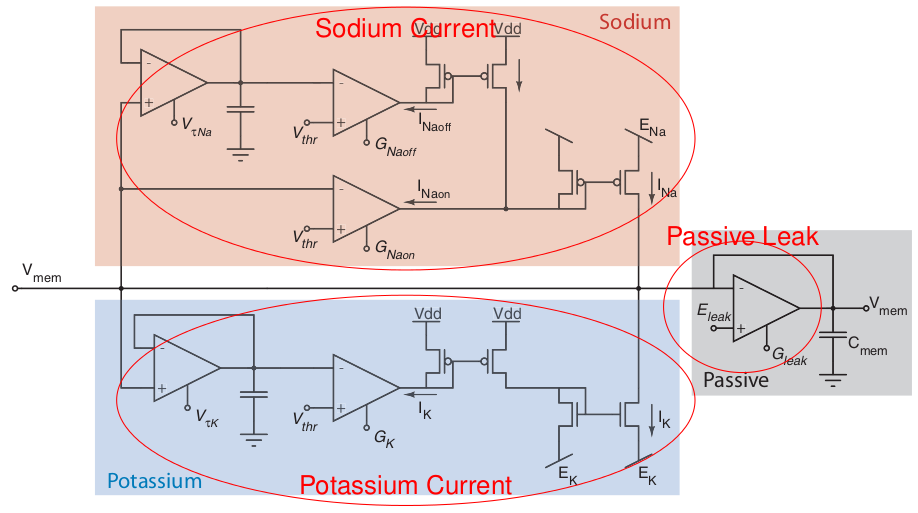
\includegraphics[width=\textwidth]{conductance-based-SI-neuron.png}
		\caption{Conductance-based silicon neuron}
	\end{subfigure}%
	~
	\begin{subfigure}[b]{0.5\textwidth}
		\centering
		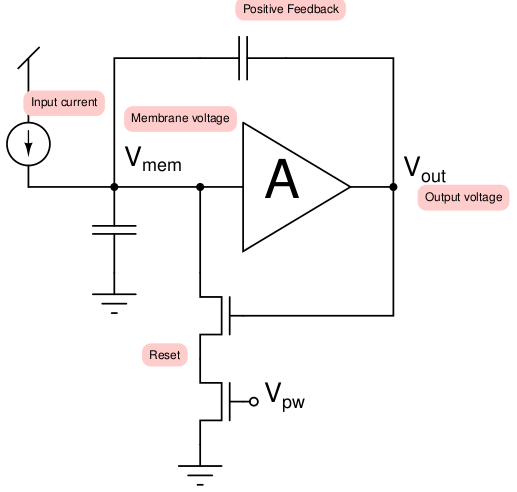
\includegraphics[width=\textwidth]{axon-hillock-circuit.png}
		\caption{Axon-Hillock-circuit}
	\end{subfigure}
\end{figure}
\begin{figure}[H]
	\centering
	\begin{subfigure}[b]{0.5\textwidth}
		\centering
		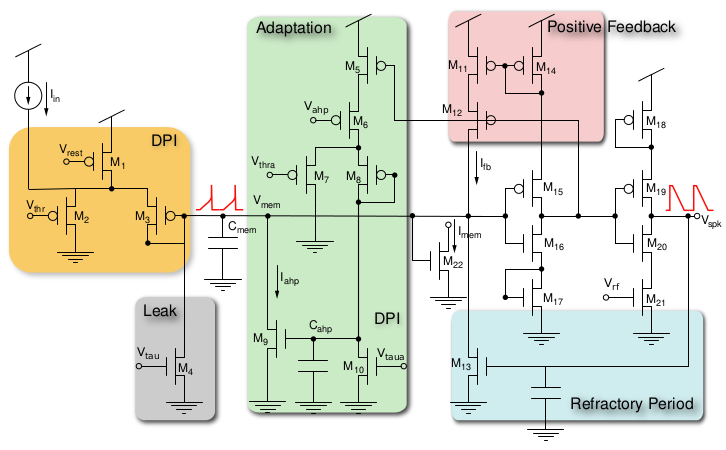
\includegraphics[width=\textwidth]{IanF-circuit.png}
		\caption{Ultra low-power generalized I\&F circuit}
	\end{subfigure}%
	~
	\begin{subfigure}[b]{0.5\textwidth}
		\centering
		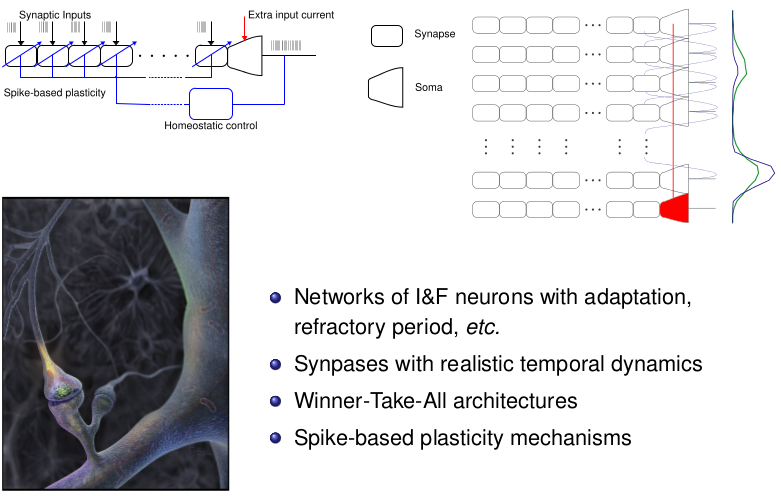
\includegraphics[width=\textwidth]{multineuron-circuit.png}
		\caption{Spiking multineuron architectures}
	\end{subfigure}
\end{figure}



\end{document}
